%%%%%%%%%%%%%%%%%%%%%%%%%%%%%%%%%%%%%%%%%
% Beamer Presentation
% LaTeX Template
% Version 1.0 (10/11/12)
%
% This template has been downloaded from:
% http://www.LaTeXTemplates.com
%
% License:
% CC BY-NC-SA 3.0 (http://creativecommons.org/licenses/by-nc-sa/3.0/)
%
%%%%%%%%%%%%%%%%%%%%%%%%%%%%%%%%%%%%%%%%%

%----------------------------------------------------------------------------------------
%	PACKAGES AND THEMES
%----------------------------------------------------------------------------------------

\documentclass{beamer}

\mode<presentation> {

% The Beamer class comes with a number of default slide themes
% which change the colors and layouts of slides. Below this is a list
% of all the themes, uncomment each in turn to see what they look like.

%\usetheme{default}
%\usetheme{AnnArbor}
%\usetheme{Antibes}
%\usetheme{Bergen}
%\usetheme{Berkeley}
%\usetheme{Berlin}
%\usetheme{Boadilla}
%\usetheme{CambridgeUS}
%\usetheme{Copenhagen}
%\usetheme{Darmstadt}
%\usetheme{Dresden}
%%\usetheme{Frankfurt}
%\usetheme{Goettingen}
%\usetheme{Hannover}
%%\usetheme{Ilmenau}
%\usetheme{JuanLesPins}
%\usetheme{Luebeck}
\usetheme{Madrid}
%\usetheme{Malmoe}
%\usetheme{Marburg}
%\usetheme{Montpellier}
%\usetheme{PaloAlto}
%\usetheme{Pittsburgh}
%\usetheme{Rochester}
%%\usetheme{Singapore}
%\usetheme{Szeged}
%\usetheme{Warsaw}

% As well as themes, the Beamer class has a number of color themes
% for any slide theme. Uncomment each of these in turn to see how it
% changes the colors of your current slide theme.

%\usecolortheme{albatross}
%\usecolortheme{beaver}
%\usecolortheme{beetle}
%\usecolortheme{crane}
%\usecolortheme{dolphin}
%\usecolortheme{dove}
%\usecolortheme{fly}
%\usecolortheme{lily}
%\usecolortheme{orchid}
%\usecolortheme{rose}
%\usecolortheme{seagull}
%\usecolortheme{seahorse}
%\usecolortheme{whale}
%\usecolortheme{wolverine}

%\setbeamertemplate{footline} % To remove the footer line in all slides uncomment this line
%\setbeamertemplate{footline}[page number] % To replace the footer line in all slides with a simple slide count uncomment this line

%\setbeamertemplate{navigation symbols}{} % To remove the navigation symbols from the bottom of all slides uncomment this line
}

\usepackage{graphicx} % Allows including images
\usepackage{booktabs} % Allows the use of \toprule, \midrule and \bottomrule in tables

\usepackage{xcolor}
\usepackage{xspace}
\usepackage{algorithm}
\usepackage{algorithmic}
\usepackage{caption}
\usepackage{multirow}

\usepackage{tikz}
\usetikzlibrary{matrix, decorations, patterns, positioning, shapes, calc, intersections, arrows, fit}
\newcommand\addvmargin[1]{
	\node[fit=(current bounding box),inner ysep=#1,inner xsep=0]{};
}

\newcommand{\tensor}[1]{{\cal\textbf{#1}\xspace}}
\newcommand{\ttrain}{{\it Tensor-Train}\xspace}

\newcommand{\hfirst}{{\it LSR}\xspace}
\newcommand{\hsecond}{{\it SLSB}\xspace}
\newcommand{\hthird}{{\it LSB}\xspace}
\newcommand{\otta}{{\it STTA}\xspace}

%% Colors from https://latexcolor.com/
\definecolor{pastelviolet}{rgb}{0.8, 0.6, 0.79}
\definecolor{babyblueeyes}{rgb}{0.63, 0.79, 0.95}
\definecolor{pastelyellow}{rgb}{0.99, 0.99, 0.59}
\definecolor{pastelgreen}{rgb}{0.47, 0.87, 0.47}
\definecolor{pastelred}{rgb}{1.0, 0.41, 0.38}
\colorlet{patternblue}{blue!60}
%----------------------------------------------------------------------------------------
%	TITLE PAGE
%----------------------------------------------------------------------------------------

\title[Parallel Tensor Train]{Parallel Tensor Train through Hierarchical Decomposition} % The short title appears at the bottom of every slide, the full title is only on the title page

\author[Suraj {\sc Kumar}]{Laura {\sc Grigori}, and \underline{Suraj {\sc Kumar}}} % Your name
\institute[Inria Paris] % Your institution as it will appear on the bottom of every slide, may be shorthand to save space
{Inria Paris % Your institution for the title page
%%\medskip
%%\textit{suraj.kumar@inria.fr} % Your email address
}
\date[ROMA Working Group]{ROMA Working Group\\ \today}

\begin{document}

\begin{frame}
\titlepage % Print the title page as the first slide
\end{frame}


\section{Introduction}
\begin{frame}
\frametitle{Overview} % Table of contents slide, comment this block out to remove it
\tableofcontents % Throughout your presentation, if you choose to use \section{} and \subsection{} commands, these will automatically be printed on this slide as an overview of your presentation
\end{frame}

%------------------------------------------------
\begin{frame}
\frametitle{Table of Contents}
\tableofcontents[currentsection]
\end{frame}

\begin{frame}{Tensors: Multidimensional Arrays}
\begin{tabular}{ccc}
Dimension & Name &\\
%%\begin{tikzpicture}[scale=0.625, every node/.style={transform shape}]
%%\tikzstyle{taskr}=[draw=black, minimum height=1mm, minimum width=12mm, anchor=south west, fill=pastelgreen, text=black]
%%			\node (t01) at (0,0) [taskr]{};
%%\end{tikzpicture}
%%\begin{tikzpicture}
%%\pgfmathsetmacro{\cubex}{5}
%%\pgfmathsetmacro{\cubey}{1}
%%\pgfmathsetmacro{\cubez}{3}
%%\draw[red,fill=yellow] (0,0,0) -- ++(-\cubex,0,0) -- ++(0,-\cubey,0) -- ++(\cubex,0,0) -- cycle;
%%\draw[red,fill=yellow] (0,0,0) -- ++(0,0,-\cubez) -- ++(0,-\cubey,0) -- ++(0,0,\cubez) -- cycle;
%%\draw[red,fill=yellow] (0,0,0) -- ++(-\cubex,0,0) -- ++(0,0,-\cubez) -- ++(\cubex,0,0) -- cycle;
%%\end{tikzpicture}
%%$0$ & Scalar & \\
$1$ & Vector & 
\begin{tikzpicture}[scale=0.25, every node/.style={transform shape}]
\pgfmathsetmacro{\rectx}{4}
\pgfmathsetmacro{\recty}{0.5}
\draw[blue,fill=pastelgreen] (0,0) -- ++(-\rectx,0) -- ++(0,\recty) -- ++(\rectx, 0) -- cycle;
\end{tikzpicture} \\
&&\\
$2$ & Matrix & 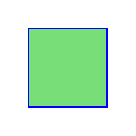
\begin{tikzpicture}[scale=0.25, every node/.style={transform shape}]
\pgfmathsetmacro{\rectx}{4}
\pgfmathsetmacro{\recty}{4}
\draw[blue,fill=pastelgreen] (0,0) -- ++(-\rectx,0) -- ++(0,\recty) -- ++(\rectx, 0) -- cycle;
%%\addvmargin{4};
\end{tikzpicture}\\
&&\\
$3$ & $3$-dimensional tensor & 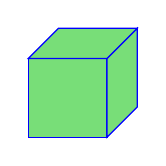
\begin{tikzpicture}[scale=0.25, every node/.style={transform shape}]
\pgfmathsetmacro{\cubex}{4}
\pgfmathsetmacro{\cubey}{4}
\pgfmathsetmacro{\cubez}{4}
\draw[blue,fill=pastelgreen] (0,0,0) -- ++(-\cubex,0,0) -- ++(0,-\cubey,0) -- ++(\cubex,0,0) -- cycle;
\draw[blue,fill=pastelgreen] (0,0,0) -- ++(0,0,-\cubez) -- ++(0,-\cubey,0) -- ++(0,0,\cubez) -- cycle;
\draw[blue,fill=pastelgreen] (0,0,0) -- ++(-\cubex,0,0) -- ++(0,0,-\cubez) -- ++(\cubex,0,0) -- cycle;
\end{tikzpicture}\\
&&\\
$4$ & $4$-dimensional tensor & 
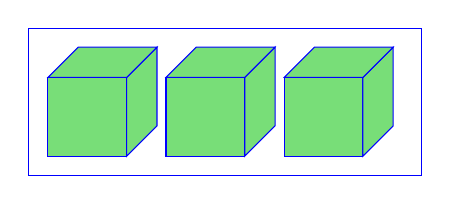
\begin{tikzpicture}[scale=0.25, every node/.style={transform shape}]
\pgfmathsetmacro{\cubex}{4}
\pgfmathsetmacro{\cubey}{4}
\pgfmathsetmacro{\cubez}{4}
\draw[blue,fill=pastelgreen] (0,0,0) -- ++(-\cubex,0,0) -- ++(0,-\cubey,0) -- ++(\cubex,0,0) -- cycle;
\draw[blue,fill=pastelgreen] (0,0,0) -- ++(0,0,-\cubez) -- ++(0,-\cubey,0) -- ++(0,0,\cubez) -- cycle;
\draw[blue,fill=pastelgreen] (0,0,0) -- ++(-\cubex,0,0) -- ++(0,0,-\cubez) -- ++(\cubex,0,0) -- cycle;

\draw[blue,fill=pastelgreen] (\cubex +2,0,0) -- ++(-\cubex,0,0) -- ++(0,-\cubey,0) -- ++(\cubex,0,0) -- cycle;
\draw[blue,fill=pastelgreen] (\cubex +2,0,0) -- ++(0,0,-\cubez) -- ++(0,-\cubey,0) -- ++(0,0,\cubez) -- cycle;
\draw[blue,fill=pastelgreen] (\cubex +2,0,0) -- ++(-\cubex,0,0) -- ++(0,0,-\cubez) -- ++(\cubex,0,0) -- cycle;

\draw[blue,fill=pastelgreen] (\cubex +2 + \cubex +2,0,0) -- ++(-\cubex,0,0) -- ++(0,-\cubey,0) -- ++(\cubex,0,0) -- cycle;
\draw[blue,fill=pastelgreen] (\cubex +2 + \cubex +2,0,0) -- ++(0,0,-\cubez) -- ++(0,-\cubey,0) -- ++(0,0,\cubez) -- cycle;
\draw[blue,fill=pastelgreen] (\cubex +2 + \cubex +2,0,0) -- ++(-\cubex,0,0) -- ++(0,0,-\cubez) -- ++(\cubex,0,0) -- cycle;

\draw[blue, fill=none] (-\cubex -1, 2.5, 0) -- ++(0, -\cubey -3.5, 0) -- ++(\cubex +2 + \cubex +2 + \cubex + \cubex,0,0) -- ++(0, \cubey +3.5, 0) -- cycle; 
\end{tikzpicture}
\end{tabular}

\end{frame}

%------------------------------------------------

\begin{frame}{Tensors}
\begin{itemize}
	\item Tensors are used in several domains
	\begin{itemize}
		\item Quantum molecular dynamics, signal processing, data mining, neurosciences, computer vision, psychometrics, chemometrics, ...
	\end{itemize}
	\vfill
	\item Memory and computation requirements are exponential in the number of dimensions
	\begin{itemize}
		\item A molecular simulation involving just $100$ spatial orbitals  manipulate a huge tensor with $4^{100}$ elements
		\item People work with low dimensional structure of the tensors
	\end{itemize}
	\vfill
	\item Limited work on parallelization of tensor algorithms
	%%    \begin{itemize}
	%%    	\item Matricized Tensor Times Khatri Rao Product (MTTKRP), tensor contraction
	%%    \end{itemize}
\end{itemize}
\end{frame}

\section{Low Rank Tensor Representations} % Sections can be created in order to organize your presentation into discrete blocks, all sections and subsections are automatically printed in the table of contents as an overview of the talk
\begin{frame}
\frametitle{Table of Contents}
\tableofcontents[currentsection]
\end{frame}

%%\begin{frame}{World}
%%content...
%%\end{frame}
\begin{frame}{Singular Value Decomposition (SVD) of Matrices}
\begin{itemize}
	\item It decomposes a matrix $A$ $\in$ $\mathbb{R}^{m \times n}$ to the form $U\Sigma V^T$
	\begin{itemize}
		\item $U$ is an $m\times m$ orthogonal matrix
		\item $V$ is an $n\times n$ orthogonal matrix
		\item $\Sigma$ is an $m\times n$ rectangular diagonal matrix
	\end{itemize}
	\item It represents a matrix as the sum of rank one matrices
	\begin{itemize}
		\item $A= \sum_i \Sigma(i;i)U_i V_i^T$
		\item Minimum number of rank one matrices required in the sum is called the rank of the original matrix
	\end{itemize}
\end{itemize}

\begin{center}
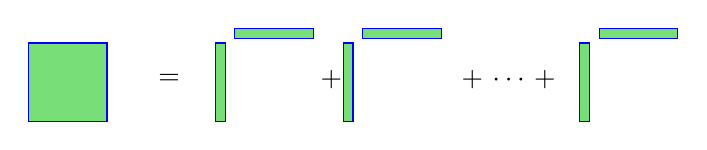
\begin{tikzpicture}[scale=0.25, every node/.style={transform shape}]
\pgfmathsetmacro{\cubex}{4}
\pgfmathsetmacro{\cubey}{4}
\pgfmathsetmacro{\cubez}{4}
\draw[blue,fill=pastelgreen] (0,0,0) -- ++(-\cubex,0,0) -- ++(0,-\cubey,0) -- ++(\cubex,0,0) -- cycle;
%%\draw[blue,fill=pastelgreen] (0,0,0) -- ++(0,0,-\cubez) -- ++(0,-\cubey,0) -- ++(0,0,\cubez) -- cycle;
%%\draw[blue,fill=pastelgreen] (0,0,0) -- ++(-\cubex,0,0) -- ++(0,0,-\cubez) -- ++(\cubex,0,0) -- cycle;

\node[draw=none, text=black, scale=4] at (2,-3,-3) {$=$};
\pgfmathsetmacro{\smallwidth}{0.5}
\draw[blue,fill=pastelgreen] (\cubex+2,0,0) -- ++(-\smallwidth,0,0) -- ++(0,-\cubey,0) -- ++(\smallwidth,0,0) -- cycle;
\draw[blue,fill=pastelgreen] (\cubex+2 +\cubex + 0.5,0.75,0) -- ++(-\cubex,0,0) -- ++(0,-\smallwidth,0) -- ++(\cubex,0,0) -- cycle;
%%\draw[blue,fill=pastelgreen] (\cubex+2,0.5,0) -- ++(-\smallwidth,0,0) -- ++(0,0,-\cubez) -- ++(\smallwidth,0,0) -- cycle;

\node[draw=none, text=black, scale=4] at (2+\cubex+4.25,-3,-3) {$+$};

\draw[blue,fill=pastelgreen] (\cubex+2.5 + \cubex+2,0,0) -- ++(-\smallwidth,0,0) -- ++(0,-\cubey,0) -- ++(\smallwidth,0,0) -- cycle;
\draw[blue,fill=pastelgreen] (\cubex+2.5+\cubex+2 +\cubex + 0.5,0.75,0) -- ++(-\cubex,0,0) -- ++(0,-\smallwidth,0) -- ++(\cubex,0,0) -- cycle;
%%\draw[blue,fill=pastelgreen] (\cubex+2.5+\cubex+2,0.5,0) -- ++(-\smallwidth,0,0) -- ++(0,0,-\cubez) -- ++(\smallwidth,0,0) -- cycle;

\node[draw=none, text=black, scale=4] at (2+\cubex+5 + \cubex+ 4.25, -3,-3) {$+$ $\cdots$ $+$};

\draw[blue,fill=pastelgreen] (12 + \cubex+2.5 + \cubex+2,0,0) -- ++(-\smallwidth,0,0) -- ++(0,-\cubey,0) -- ++(\smallwidth,0,0) -- cycle;
\draw[blue,fill=pastelgreen] (12+\cubex+2.5+\cubex+2 +\cubex + 0.5,0.75,0) -- ++(-\cubex,0,0) -- ++(0,-\smallwidth,0) -- ++(\cubex,0,0) -- cycle;
%%\draw[blue,fill=pastelgreen] (12 + \cubex+2.5+\cubex+2,0.5,0) -- ++(-\smallwidth,0,0) -- ++(0,0,-\cubez) -- ++(\smallwidth,0,0) -- cycle;
\end{tikzpicture}
\end{center}
\end{frame}
\begin{frame}{Popular Tensor Decompositions}{Higher Order Generalization of SVD}
\begin{itemize}
	\item Canonical decomposition (equivalently known as Canonical Polyadic or CANDECOMP or PARAFAC)
	\vfill
	\item Tucker decomposition
	\vfill
	\item Tensor Train decomposition (equivalently known as Matrix Product States)
	\vfill
\end{itemize}
\begin{block}{Tensor Notations}
	\begin{itemize}
		\item \tensor{A} $\in \mathbb{R}^{n_1 \times \ldots \times n_d}$ is a $d$-dimensional tensor
		\item $\tensor{A}(i_1,\cdots,i_d)$ represent elements of $\tensor{A}$
		\item Use bold letters to denote tensors
	\end{itemize}
\end{block}
\end{frame}

\begin{frame}{Canonical Representation}
\begin{center}
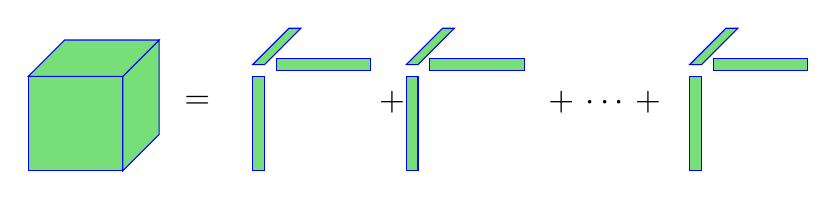
\begin{tikzpicture}[scale=0.3, every node/.style={transform shape}]
\pgfmathsetmacro{\cubex}{4}
\pgfmathsetmacro{\cubey}{4}
\pgfmathsetmacro{\cubez}{4}
\draw[blue,fill=pastelgreen] (0,0,0) -- ++(-\cubex,0,0) -- ++(0,-\cubey,0) -- ++(\cubex,0,0) -- cycle;
\draw[blue,fill=pastelgreen] (0,0,0) -- ++(0,0,-\cubez) -- ++(0,-\cubey,0) -- ++(0,0,\cubez) -- cycle;
\draw[blue,fill=pastelgreen] (0,0,0) -- ++(-\cubex,0,0) -- ++(0,0,-\cubez) -- ++(\cubex,0,0) -- cycle;

\node[draw=none, text=black, scale=4] at (2,-2.25,-3) {$=$};
\pgfmathsetmacro{\smallwidth}{0.5}
\draw[blue,fill=pastelgreen] (\cubex+2,0,0) -- ++(-\smallwidth,0,0) -- ++(0,-\cubey,0) -- ++(\smallwidth,0,0) -- cycle;
\draw[blue,fill=pastelgreen] (\cubex+2 +\cubex + 0.5,0.75,0) -- ++(-\cubex,0,0) -- ++(0,-\smallwidth,0) -- ++(\cubex,0,0) -- cycle;
\draw[blue,fill=pastelgreen] (\cubex+2,0.5,0) -- ++(-\smallwidth,0,0) -- ++(0,0,-\cubez) -- ++(\smallwidth,0,0) -- cycle;

\node[draw=none, text=black, scale=4] at (2+\cubex+4.25,-2.25,-3) {$+$};

\draw[blue,fill=pastelgreen] (\cubex+2.5 + \cubex+2,0,0) -- ++(-\smallwidth,0,0) -- ++(0,-\cubey,0) -- ++(\smallwidth,0,0) -- cycle;
\draw[blue,fill=pastelgreen] (\cubex+2.5+\cubex+2 +\cubex + 0.5,0.75,0) -- ++(-\cubex,0,0) -- ++(0,-\smallwidth,0) -- ++(\cubex,0,0) -- cycle;
\draw[blue,fill=pastelgreen] (\cubex+2.5+\cubex+2,0.5,0) -- ++(-\smallwidth,0,0) -- ++(0,0,-\cubez) -- ++(\smallwidth,0,0) -- cycle;

\node[draw=none, text=black, scale=4] at (2+\cubex+5 + \cubex+ 4.25, -2.25,-3) {$+$ $\cdots$ $+$};

\draw[blue,fill=pastelgreen] (12 + \cubex+2.5 + \cubex+2,0,0) -- ++(-\smallwidth,0,0) -- ++(0,-\cubey,0) -- ++(\smallwidth,0,0) -- cycle;
\draw[blue,fill=pastelgreen] (12+\cubex+2.5+\cubex+2 +\cubex + 0.5,0.75,0) -- ++(-\cubex,0,0) -- ++(0,-\smallwidth,0) -- ++(\cubex,0,0) -- cycle;
\draw[blue,fill=pastelgreen] (12 + \cubex+2.5+\cubex+2,0.5,0) -- ++(-\smallwidth,0,0) -- ++(0,0,-\cubez) -- ++(\smallwidth,0,0) -- cycle;

\end{tikzpicture}
\end{center}

\begin{itemize}
	\item $\tensor{A}(i_1,\cdots,i_d) = \sum_{\alpha=1}^{r} U_1(i_1,\alpha) U_2(i_2,\alpha)\cdots U_d(i_d,\alpha)$
%%	\item The minimum value of $r$ is called the canonical rank
\end{itemize}
\medspace
\begin{itemize}
	\item ({\color{green}+})  For $n_1=n_2=\cdots n_d=n$, the number of entries = $\mathcal{O}(nrd)$
	\item ({\color{red}-}) Determining the minimum value of $r$ is an NP-complete problem
	\item ({\color{red}-}) No robust algorithms to compute this representation
\end{itemize}
\end{frame}

\begin{frame}{Tucker Representation}
\begin{center}
	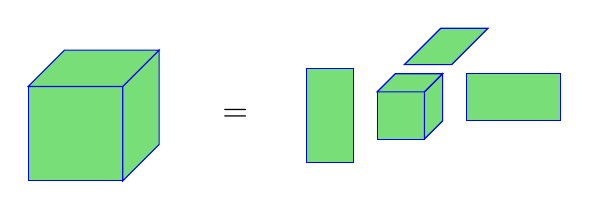
\begin{tikzpicture}[scale=0.3, every node/.style={transform shape}]
	\pgfmathsetmacro{\cubex}{4}
	\pgfmathsetmacro{\cubey}{4}
	\pgfmathsetmacro{\cubez}{4}
	\draw[blue,fill=pastelgreen] (-12,1,\cubez-2) -- ++(-\cubex,0,0) -- ++(0,-\cubey,0) -- ++(\cubex,0,0) -- cycle;
	\draw[blue,fill=pastelgreen] (-12,1,\cubez-2) -- ++(0,0,-\cubez) -- ++(0,-\cubey,0) -- ++(0,0,\cubez) -- cycle;
	\draw[blue,fill=pastelgreen] (-12,1,\cubez-2) -- ++(-\cubex,0,0) -- ++(0,0,-\cubez) -- ++(\cubex,0,0) -- cycle;
	\node[draw=none, text=black, scale=4] at (-8,-1,0) {$=$};

	\pgfmathsetmacro{\cubex}{2}
	\pgfmathsetmacro{\cubey}{2}
	\pgfmathsetmacro{\cubez}{2}
	\draw[blue,fill=pastelgreen] (0,0,0) -- ++(-\cubex,0,0) -- ++(0,-\cubey,0) -- ++(\cubex,0,0) -- cycle;
	\draw[blue,fill=pastelgreen] (0,0,0) -- ++(0,0,-\cubez) -- ++(0,-\cubey,0) -- ++(0,0,\cubez) -- cycle;
	\draw[blue,fill=pastelgreen] (0,0,0) -- ++(-\cubex,0,0) -- ++(0,0,-\cubez) -- ++(\cubex,0,0) -- cycle;
	
	\draw[blue,fill=pastelgreen] (-\cubex-1,1,0) -- ++(-\cubex,0,0) -- ++(0,-\cubey-2,0) -- ++(\cubex,0,0) -- cycle;
	\draw[blue,fill=pastelgreen] (\cubex+2+1,0,-\cubey) -- ++(-\cubex-2,0,0) -- ++(0,-\cubey,0) -- ++(\cubex+2,0,0) -- cycle;
	
	\draw[blue,fill=pastelgreen] (0,0,-\cubez-1) -- ++(-\cubex,0,0) -- ++(0,0,-\cubez-2) -- ++(\cubex,0,0) -- cycle;
	\end{tikzpicture}
\end{center}

\begin{itemize}
	\item Represents a tensor with $d$ matrices and a small core tensor
	\item $\tensor{A}(i_1,\cdots,i_d) = \sum_{\alpha_1=1}^{r_1}\cdots\sum_{\alpha_d=1}^{r_d} \tensor{g}_{\alpha_1\cdots\alpha_d}U_1(i_1,\alpha_1)$ $\cdots U_d(i_d, \alpha_d)$
	\medspace
\end{itemize}
\medspace
\begin{itemize}
\item ({\color{green}+}) SVD based stable algorithms to compute this representation
\item ({\color{red}-})  For $n_1=n_2=\cdots n_d=n$ and $r_1=r_2=\cdots =r_d=r$, the number of entries = $\mathcal{O}(ndr+r^d)$
\end{itemize}	
\end{frame}

%------------------------------------------------
\begin{frame}{Tensor Train Representation: Product of Matrices View}
\begin{itemize}
	\item A $d$-dimensional tensor is represented with $2$ matrices and $d$-$2$ $3$-dimensional tensors.
\end{itemize}
\begin{figure}
	\begin{center}	
		\includegraphics[scale=0.35]{./diagrams/ttentry.eps}
	\end{center}
\end{figure}
\noindent An entry of $\tensor{A}$ $\in$ $\mathbb{R}^{n_1 \times \cdots \times n_d}$ is computed by multiplying corresponding matrix (or row/column) of each core.
\end{frame}

\begin{frame}{Tensor Train Representation}

\begin{block}{}
	$\tensor{A}$ $\in$ $\mathbb{R}^{n_1 \times \cdots \times n_d}$ is represented with cores $\tensor{G}_k$$\in$ $\mathbb{R}^{r_{k-1}\times n_k\times r_k}$, $k$=$1,2,\cdots d$, $r_0$=$r_d$=$1$ and its elements satisfy the following expression:
	{\small\begin{align*}
		\tensor{A}(i_1,\cdots ,i_d) 
		&= \sum_{\alpha_0 = 1}^{r_0} \cdots \sum_{\alpha_d = 1}^{r_d} \tensor{G}_1(\alpha_0, i_1, \alpha_1) \cdots \tensor{G}_d(\alpha_{d-1}, i_d, \alpha_d)\\
		&= \sum_{\alpha_1 = 1}^{r_1} \cdots \sum_{\alpha_{d-1} = 1}^{r_{d-1}} \tensor{G}_1(1, i_1, \alpha_1) \cdots \tensor{G}_d(\alpha_{d-1}, i_d, 1)
		\end{align*}}
	\begin{center}
	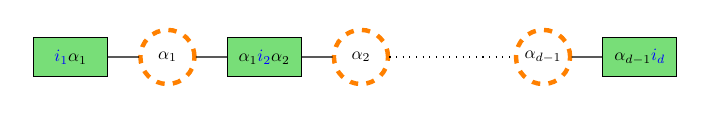
\begin{tikzpicture}[scale=0.625, every node/.style={transform shape}]
	\tikzstyle{taskc}=[circle, draw=orange, minimum size=11mm, fill=none, dashed, ultra thick]
	\tikzstyle{taskr}=[draw=black, minimum height=8mm, minimum width=15mm, anchor=south west, fill=pastelgreen, text=black]
	
	\node(t1) at (0,0) {};
	\node [above right=0cm and 0cm of t1.mid,taskr](T1) {$\textcolor{blue}{i_1}\alpha_1$};
	\node [above right=0cm and 0.8cm of T1.south east, taskc](C1) {$\alpha_1$};
	\node [above right=0cm and 0.8cm of C1.south east, taskr](T2) {$\alpha_1\textcolor{blue}{i_2}\alpha_2$};
	\node [above right=0cm and 0.8cm of T2.south east, taskc](C2) {$\alpha_2$};
	
	\node [above right=0cm and 4.5cm of T2.south east, taskc](Cd) {$\alpha_{d\text{-}1}$};
	\node [above right=0cm and 0.8cm of Cd.south east, taskr](Td) {$\alpha_{d\text{-}1}\textcolor{blue}{i_d}$};
	\draw (T1.east)--(C1.west);
	\draw (C1.east)--(T2.west);
	\draw (T2.east)--(C2.west);
	\draw [dotted] (C2.east)--(Cd.west);
	\draw (Cd.east)--(Td.west);
	\path (-0.1, -0.4) -- (2.5, -0.4); 
	%%\path (-0.1, -0.8) -- (2.5, -0.8); 
	\end{tikzpicture}
		\end{center}
\end{block}
	\begin{itemize}
	\item For $n_1=n_2=\cdots=n_d=n$ and $r_1=r_2=\cdots=r_{d-1}=r$, the number of entries = $\mathcal{O}(ndr^2)$
\end{itemize}
\end{frame}

\section{Algorithms to Compute Tensor Train Representation}
\subsection{Sequential Algorithms}
\begin{frame}
\frametitle{Table of Contents}
\tableofcontents[currentsubsection]
\end{frame}
\begin{frame}{Unfolding Matrices of a Tensor \& Notations}
\begin{itemize}
	\item Frobenius norm of a matrix $A$ is defined as, $||A||_F = \sqrt{\sum_{i,j} A(i;j)^2}$
	\item Frobenius norm of a $d$-dimensional tensor \tensor{A} is defined as, $||\tensor{A}||_F=$ $\sqrt{\sum_{i_1, i_2, \cdots, i_d}\tensor{A}(i_1,i_2,\cdots, i_d)^2 }$
\end{itemize}
\begin{block}{$k$-th unfolding matrix}
$A_k$ denotes $k$-th unfolding matrix of tensor $\tensor{A}$ $\in$ $\mathbb{R}^{n_1 \times \cdots \times n_d}$.

$\qquad\qquad A_k = [A_k(i_1, i_2,\cdots, i_k; i_{k+1},\cdots ,i_d)]$

\begin{itemize}
	\item Size of $A_k$ is $(\prod_{l=1}^{k}n_l)\times(\prod_{l=k+1}^{d}n_l)$
	\item $r_k$ denotes the rank of $A_k$.
\end{itemize}
\end{block}
\begin{itemize}
	\item ($r_1, r_2,\cdots, r_{d-1}$) denotes the ranks of unfolding matrices of the tensor.
\end{itemize}
\end{frame}



\begin{frame}{Tensor Train Decomposition (Oseledets's Algorithm)}
\begin{algorithm}[H]
	\caption{\label{alg:tt-decomposition}Tensor Train Decomposition}
	\begin{algorithmic}[1]
		\REQUIRE $d$-dimensional tensor \tensor{A} and ranks ($r_1, r_2,\cdots r_{d-1}$) 
		\ENSURE Cores $\tensor{G}_k(\alpha_{k-1}, n_k, \alpha_k) _{1\le k\le d}$ of the Tensor Train representation with $\alpha_k \le r_k$ and $\alpha_0 = \alpha_d=1$
		%%Compute truncation parameter δ = √ d−1
		%%||A|| F .
		%%Temporary tensor: C = A, r 0 = 1.
		%%for k = 1 to d − 1 do
		%%C := reshape(C, [r k−1 n k , numel(C)
		%%r k−1 n k ]).
		%%Compute δ-truncated SVD: C = U SV + E, ||E|| F ≤ δ, r k = rank δ (C).
		%%New core: G k := reshape(U, [r k−1 , n k , r k ]).
		%%C := SV  .
		%%end for
		%%G d = C.
		%%Return tensor B in TT-format with cores G 1 , . . . , G d .
		\STATE Temporary tensor: $\tensor{C} = \tensor{A}$, $\alpha_0=1$
		\FOR{$k=1:d-1$}
		\STATE $A_k$ = $reshape(\tensor{C}, \alpha_{k-1}n_{k} , \frac{numel(\tensor{C})}{\alpha_{k-1}n_{k}})$
%%		\STATE Compute unfolding matrix $A_k$ 
		\STATE Compute SVD: $A_k = U \Sigma V^T$
		\STATE Compute rank of $\Sigma$, $\alpha_k=$ rank($\Sigma$)
		\STATE New core: $\tensor{G}_k$ := $reshape(U(;1:\alpha_k), \alpha_{k-1}, n_k, \alpha_k)$
		\STATE $\tensor{C}$ = $\Sigma(1:\alpha_k; 1:\alpha_k)V^T(1:\alpha_k;)$
		\ENDFOR
		\STATE $\tensor{G}_d$ = \tensor{C}, $\alpha_{d}=1$
		\STATE return $\tensor{G}_1,\cdots,\tensor{G}_d$
	\end{algorithmic}
\end{algorithm}
\end{frame}

\begin{frame}{Tensor Train Approximation (Oseledets's Algorithm)}
\begin{algorithm}[H]
	\caption{\label{alg:tt-approximation}Tensor Train Approximation}
	\begin{algorithmic}[1]{\small
			\REQUIRE $d$-dimensional tensor \tensor{A} and expected accuracy $\epsilon$ 
			\ENSURE Cores $\tensor{G}_k(\alpha_{k-1}, n_k, \alpha_k) _{1\le k\le d}$ of the approximated tensor \tensor{B} in Tensor Train representation such that $||\tensor{A}-\tensor{B}||_F$ is not more than $\epsilon$
			\STATE Temporary tensor: $\tensor{C} = \tensor{A}$, $\alpha_0=1$, $\delta$ = $\frac{\epsilon}{\sqrt{d-1}}$
			\FOR{$k=1:d-1$}
			\STATE $A_k$ = $reshape(\tensor{C}, \alpha_{k-1}n_{k} , \frac{numel(\tensor{C})}{\alpha_{k-1}n_{k}})$
			%%		\STATE Compute unfolding matrix $A_k$ 
			\STATE Compute SVD: $A_k = U \Sigma V^T$
			\STATE Compute $\alpha_k$ such that $A_k = U(;1:\alpha_k) \Sigma(1:\alpha_k; 1:\alpha_k) V^T(1:\alpha_k;) + E_k$ and $||E_K||_F \le \delta$
			\STATE New core: $\tensor{G}_k$ := $reshape(U(;1:\alpha_k), r_{k-1}, n_k, r_k)$
			\STATE $\tensor{C}$ = $\Sigma(1:\alpha_k; 1:\alpha_k)V^T(1:\alpha_k;)$
			\ENDFOR
			\STATE $\tensor{G}_d$ = \tensor{C}, $\alpha_{d}=1$
			\STATE return $\tensor{B}$ in Tensor Train representation with cores $\tensor{G}_1,\cdots,\tensor{G}_d$
	}\end{algorithmic}
\end{algorithm}
\end{frame}

%%\begin{frame}{Ranks of Tensor Train Representation Obtained by Algorithm~\ref{alg:tt-decomposition}}
%%\begin{block}{}
%%	\begin{center}
%%	$\alpha_{k}$ $\le$ Rank($A_k$)
%%	\end{center}
%%\end{block}
%%\end{frame}

\begin{frame}{Separatation of Dimensions \only<1>{in Sequential Algorithms}\only<2>{for Maximum Parallelization}}
\begin{block}{}
	\onslide<1->{
		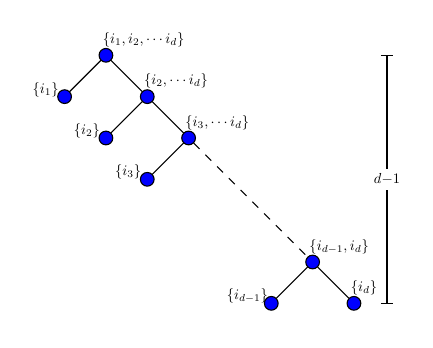
\begin{tikzpicture}[scale=0.525, every node/.style={transform shape}]
	%%\draw[fill=cyan] (0,0) circle (0.8cm);
	%%		\node [draw,circle]{r};
	%%		\tikzstyle{task}=[circle, draw, minimum size=10mm]
	%%		\node (d) at (0,0)[task, fill=babyblueeyes] {$D$};
	%%		\node (e) at (2.5,0)[task, fill=pastelviolet] {$E$};
	%%		\draw[thick, ->] (d.east) -- (e);
	%%		
	%%		\node (a) at (0,2)[task, fill=pastelyellow] {$A$};
	%%		\node (b) at (2.5,2.75)[task, fill=pastelgreen] {$B$};
	%%		\node (c) at (2.5,1.25)[task, fill=pastelred] {$C$};
	%%		
	%%		\draw[thick, ->] (a.east) -- (b);
	%%		\draw[thick, ->] (a.east) -- (c);
	\tikzstyle{taskc}=[circle, draw=black, minimum size=2mm, fill=blue]
	\tikzstyle{taskr}=[draw=none, minimum height=2mm, minimum width=5mm, anchor=south west, fill=none, text=black]
	%%
	\node (t01) at (0,0) [taskc]{};
	\node (t11) at (-1,-1) [taskc] {};
	\node (t12) at (1, -1) [taskc] {};
	\node (t21) at (0, -2) [taskc] {};
	\node (t22) at (2, -2) [taskc] {};
	\node (t31) at (1,-3) [taskc] {};
	\node (t52) at (5, -5) [taskc] {};
	\node (t61) at (4, -6) [taskc] {};
	\node (t62) at (6, -6) [taskc] {};
	
	\draw (t01) -- (t11);
	\draw (t01) -- (t12);
	\draw (t12) -- (t21);
	\draw (t12) -- (t22);
	\draw (t22) -- (t31);
	\draw [dashed] (t22) -- (t52);
	\draw (t52) -- (t61);
	\draw (t52) -- (t62);
	
	\draw (6.8, -6) -- (6.8, -3.25);
	\draw (6.8, -2.75) -- (6.8, 0);
	
	\draw (6.65, -6) -- (6.95, -6);
	\draw (6.65, -0) -- (6.95, 0);
	\node at (6.8, -3) {$d\text{-}1$};
	
	\node [above left=0mm and 2mm of t01.mid, taskr](l01) {$\{i_1,i_2,\cdots i_d\}$};
	\node [below left=2mm and 9mm of t11.mid, taskr](l11) {$\{i_1\}$};
	\node [above left=0mm and 2mm of t12.mid, taskr](l12) {$\{i_2,\cdots i_d\}$};
	\node [below left=2mm and 9mm of t21.mid, taskr](l21) {$\{i_2\}$};
	\node [above left=0mm and 2mm of t22.mid, taskr](l22) {$\{i_3,\cdots i_d\}$};
	\node [below left=2mm and 9mm of t31.mid, taskr](l31) {$\{i_3\}$};
	
	\node [above left=0mm and 2mm of t52.mid, taskr](l52) {$\{i_{d\text{-}1}, i_d\}$};
	\node [below left=2mm and 12mm of t61.mid, taskr](l61) {$\{i_{d\text{-}1}\}$};
	\node [above left=0mm and 2mm of t62.mid, taskr](l62) {$\{i_d\}$};
	
	\path (-0.1, -6.4) -- (2.5, -6.4); 
	\end{tikzpicture}
}
	\onslide<2->{
		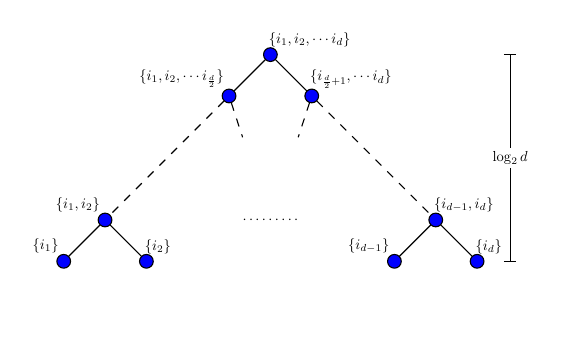
\begin{tikzpicture}[scale=0.525, every node/.style={transform shape}]
		
		\tikzstyle{taskc}=[circle, draw=black, minimum size=2mm, fill=blue]
		%%	\tikzstyle{taskr}=[draw=none, minimum height=2mm, minimum width=5mm, anchor=south west, fill=none, text=black]
		
		
		\node (t01) at (0,0) [taskc]{};
		\node (t11) at (-1,-1) [taskc] {};
		\node (t12) at (1, -1) [taskc] {};
		
		\node (tinter1) at (-0.5,-2) [taskc, draw=none, fill=none] {};
		\node (tinter2) at (0.5,-2) [taskc, draw=none, fill=none] {};
		
		\node (t41) at (-4,-4) [taskc] {};
		\node (t42) at (4,-4) [taskc] {};
		\node (t51) at (-5,-5) [taskc] {};
		\node (t52) at (-3,-5) [taskc] {};
		\node (t53) at (3,-5) [taskc] {};
		\node (t54) at (5,-5) [taskc] {};
		
		
		\draw (t01) -- (t11);
		\draw (t01) -- (t12);
		
		\draw [dashed] (t11) -- (tinter1.west);
		\draw [dashed] (t12) -- (tinter2.east);
		
		\draw [dashed] (t11) -- (t41);
		\draw [dashed] (t12) -- (t42);
		
		\path (t41) -- (t42) node [midway] {$\cdots\cdots\cdots$};
		
		\draw (t41) -- (t51);
		\draw (t41) -- (t52);
		
		\draw (t42) -- (t53);
		\draw (t42) -- (t54);
		
		
		\draw (5.8, -5) -- (5.8, -2.75);
		\draw (5.8, -2.25) -- (5.8, 0);
		
		\draw (5.65, -5) -- (5.95, -5);
		\draw (5.65, 0) -- (5.95, 0);
		\node at (5.8, -2.5) {$\log_2 d$};
		
		\node [above right] at (t01.160) {$\{i_1,i_2,\cdots i_d\}$};	
		
		\node [above left] at (t11.mid) {$\{i_1,i_2,\cdots i_\frac{d}{2}\}$};	
		\node [above right] at (t12.160) {$\{i_{\frac{d}{2}+1},\cdots i_d\}$};
		
		\node [above left] at (t41.mid) {$\{i_1,i_2\}$};
		\node [above right] at (t42.160) {$\{i_{d-1}, i_d\}$};
		
		\node [above left] at (t51.mid) {$\{i_1\}$};
		\node [above right] at (t52.160) {$\{i_2\}$};
		
		\node [above left] at (t53.mid) {$\{i_{d-1}\}$};
		\node [above right] at (t54.160) {$\{i_d\}$};
		
		
		\path (-0.1, -6.4) -- (2.5, -6.4); 
		%%		\path (-6.5, 0) -- (0,0);
		\end{tikzpicture}
	}
\end{block}
\end{frame}

\subsection{Parallel Algorithms}
\begin{frame}
\frametitle{Table of Contents}
\tableofcontents[currentsubsection]
\end{frame}

\begin{frame}{Extra Definitions for Parallel Algorithms}
\begin{itemize}
	\item Original indices of a tensor are called external indices
	\item Indices obtained due to SVD are called internal indices
	\begin{itemize}
		\item $\tensor{A}(\alpha, i_1, i_2, i_3, \beta)$ has $3$ external and $2$ internal indices
	\end{itemize}
	\item $nEI(\tensor{A})$ denotes the number of external indices of \tensor{A}
\end{itemize}
\begin{block}{$k$-th Unfolding Matrix}
 $k$-th unfolding of a tensor with elements $\tensor{A}(\alpha, i_1, i_2, \cdots,i_k, i_{k+1}, \cdots, \beta)$ is represented as, $ A_k = [A_k(\alpha, i_1, i_2, \cdots, i_k; i_{k+1}\cdots, \beta)]$.
 
\medskip
	\noindent All indices from the beginning to $i_{k}$ denote the rows of $A_k$ and the remaining indices denote the columns of $A_k$.
\end{block}
\begin{itemize}
	\item \textbf{Tensor}($A_l$) converts an unfolding matrix $A_l$ to its tensor form
\end{itemize}
\end{frame}

\begin{frame}[allowframebreaks]{Parallel Tensor Train decomposition}
%%\begin{algorithm}[H]
	\rule{\textwidth}{0.5pt}
	\captionof{algorithm}{\label{alg:tt_parallel}PTT-decomposition (parallel Tensor Train Decomposition)}%
	\vspace*{-0.5cm}
	\rule{\textwidth}{0.5pt}%
	\vspace*{-0.5cm}
%%	\caption{\label{alg:tt_parallel}Parallel Tensor Train Decomposition}
	\begin{algorithmic}[1]
		\REQUIRE $d$-dimensional tensor \tensor{A} and ranks ($r_1, r_2,\cdots r_{d-1}$) 
		\ENSURE Cores $\tensor{G}_k(\alpha_{k-1}, n_k, \alpha_k) _{1\le k\le d}$ of the Tensor Train representation with $\alpha_k \le r_k$ and $\alpha_0 = \alpha_d=1$
		\IF{$nEI(\tensor{A})> $$1$} 
		\STATE Find the middle external index $k$
		\STATE Compute unfolding matrix $A_k$ 
		\STATE Compute SVD: $A_k = U \Sigma V^T$
		\STATE Compute rank of $\Sigma$, $\alpha_k=$ rank($\Sigma$)
		\STATE Select diagonal matrices $X_k$, $S_k$ and $Y_k$ such that $X_kS_kY_k = \Sigma(1:\alpha_k; 1:\alpha_k)$\label{alg:line:xsy}
		%%		\STATE // first $\alpha_k$ columns of $U$
		\STATE $\tensor{A}$$_{left}$ = \textbf{Tensor}($U(;1:\alpha_k)X_k$)
		\STATE list1 = PTT-decomposition($\tensor{A}$$_{left}$, ($r_1,\cdots r_{k-1},\alpha_k$) )
		\STATE $\tensor{A}$$_{right}$ = \textbf{Tensor}($Y_kV^T(1:\alpha_k;)$)
		\STATE list2= PTT-decomposition($\tensor{A}$$_{right}$,($\alpha_k, r_{k+1},\cdots r_{d-1}$))
		\RETURN \{list1, list2\}
		\ELSE 
		\STATE Find the external index $k$
		\IF {$k$ is the last index of \tensor{A}} 
		\STATE $\alpha_k = 1$
		%%		\ENDIF
		\ELSIF {$k$ is the first index of \tensor{A}}
		\STATE $\alpha_{k\text{-}1} = 1$
		\STATE $\tensor{A}(i_k, \beta)$ = $\sum_{\beta=1}^{\alpha_k} \tensor{A}(i_k, \beta)S_k(\beta;\beta)$ \label{alg:ptt:firstcore}
		\ELSE
		\STATE $ \tensor{A}(\gamma, i_k, \beta)$ = $\sum_{\beta=1}^{\alpha_k} \tensor{A}(\gamma, i_k, \beta)S_k(\beta;\beta)$\label{alg:ptt:otherthanfirstcore}
		\ENDIF
		\STATE $\tensor{G}_k$ = $ \tensor{A}$
		\STATE return $\tensor{G}_k$
		\ENDIF
	\end{algorithmic}
%%\end{algorithm}
\end{frame}

\begin{frame}{Diagramatic Representation of the Algorithm}
	\begin{center}
	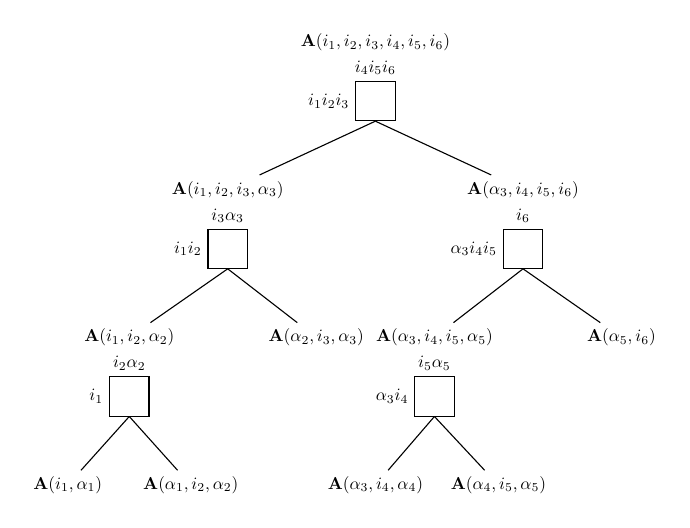
\begin{tikzpicture}[scale=0.625, every node/.style={transform shape}]
	\tikzstyle{taskr}=[draw=black, minimum height=8mm, minimum width=8mm, fill=none, text=black]
	%%	anchor=south west,
	\node (t10) at (0,1.2) {$\tensor{A}(i_1,i_2,i_3,i_4,i_5,i_6)$};	
	\node (b01) at (0,0) [taskr]{};
	\node [above] at (b01.north) {$i_4i_5i_6$};
	\node [left] at (b01.west) {$i_1i_2i_3$};		
	
	\node (t11) at (-3,-1.8) {$\tensor{A}(i_1,i_2,i_3,\alpha_3)$};
	\node (t12) at (3,-1.8) {$\tensor{A}(\alpha_3, i_4, i_5, i_6)$};
	
	\draw (b01.south) -- (t11);	
	\draw (b01.south) -- (t12);
	
	\node (b11) at (-3,-3) [taskr]{};
	\node (b12) at (3,-3) [taskr]{};
	
	\node [above] at (b11.north) {$i_3\alpha_3$};
	\node [left] at (b11.west) {$i_1i_2$};
	
	\node [above] at (b12.north) {$i_6$};
	\node [left] at (b12.west) {$\alpha_3i_4i_5$};
	
	\node (t21) at (-5, -4.8) {$\tensor{A}(i_1,i_2,\alpha_2)$};
	\node (t22) at (-1.2, -4.8) {$\tensor{A}(\alpha_2, i_3,\alpha_3)$};
	
	\node (t23) at (1.2, -4.8) {$\tensor{A}(\alpha_3,i_4,i_5,\alpha_5)$};
	\node (t24) at (5, -4.8) {$\tensor{A}(\alpha_5, i_6)$};
	
	\draw (b11.south) -- (t21);
	\draw (b11.south) -- (t22);
	
	\draw (b12.south) -- (t23);
	\draw (b12.south) -- (t24);		
	
	\node (b21) at (-5,-6) [taskr]{};
	\node [above] at (b21.north) {$i_2\alpha_2$};
	\node [left] at (b21.west) {$i_1$};
	
	\node (b22) at (1.2,-6) [taskr]{};
	\node [above] at (b22.north) {$i_5\alpha_5$};
	\node [left] at (b22.west) {$\alpha_3i_4$};
	
	\node (t31) at (-6.25, -7.8) {$\tensor{A}(i_1,\alpha_1)$};
	\node (t32) at (-3.75, -7.8) {$\tensor{A}(\alpha_1,i_2,\alpha_2)$};
	
	\draw (b21.south) -- (t31);
	\draw (b21.south) -- (t32);
	
	\node (t33) at (0, -7.8) {$\tensor{A}(\alpha_3,i_4,\alpha_4)$};
	\node (t34) at (2.5, -7.8) {$\tensor{A}(\alpha_4,i_5,\alpha_5)$};
	
	\draw (b22.south) -- (t33);
	\draw (b22.south) -- (t34);
	
	\end{tikzpicture}
\end{center}
\end{frame}

\begin{frame}{Ranks of Tensor Train Representation (Algorithm~\ref{alg:tt_parallel})}
%%\begin{block}{}
	\vspace*{-0.25cm}\begin{theorem}{\small
		If for each unfolding $A_k$ of a $d$-dimensional tensor \tensor{A}, $rank(A_k)=r_k$, then Algorithm~\ref{alg:tt_parallel} produces a Tensor Train representation with ranks not higher than $r_k$.}
	\end{theorem}
%%	\begin{center}
%%		$\alpha_{k}$ $\le$ Rank($A_k$)
%%	\end{center}
%%\end{block}
{\scriptsize The rank of the $k$th-unfolding matrix is $r_k$; hence it can be written as:\begin{align*}
A_k(i_1,\cdots,i_k;i_{k+1},\cdots, i_d)
&= \sum_{\alpha=1}^{r_k} U(i_1,\cdots,i_k; \alpha)\Sigma(\alpha; \alpha)V^T(\alpha;i_{k+1},\cdots, i_d)\\
&= \sum_{\alpha=1}^{r_k} U(i_1,\cdots,i_k; \alpha)X(\alpha; \alpha)S(\alpha; \alpha)Y(\alpha; \alpha) V^T(\alpha;i_{k+1},\cdots, i_d)\\
&= \sum_{\alpha=1}^{r_k} B(i_1,\cdots,i_k; \alpha)S(\alpha; \alpha)C(\alpha;i_{k+1},\cdots, i_d).
\end{align*}
In matrix form we obtain, $
A_k = BSC, B = A_k C^{-1}S^{-1} = A_kZ, C = S^{-1}B^{-1}A_k = WA_k$.\\
%%	\quad B = A_k (C^T)^{-1}S^{-1} &= A_kZ\\
%%	\quad C = A_k^T (B^T)^{-1}S^{-1} &= A_k^T W
\noindent or in the index form, $B(i_1,\cdots, i_k; \alpha) = \sum_{i_{k+1}=1}^{n_{k+1}}\cdots\sum_{i_d=1}^{n_d} \tensor{A}(i_1, \cdots, i_d) Z(i_{k+1},\cdots, i_d;\alpha),$\\
	$\qquad C(\alpha; i_{k+1},\cdots, i_d) = \sum_{i_1=1}^{n_1} \cdots \sum_{i_k=k}^{n_k} \tensor{A}(i_1, \cdots, i_d) W(\alpha;i_1,i_2,\cdots, i_k)$.
	
\noindent $B$ and $C$ can be treated as $k+1$ and $d$-$k+1$ dimensional tensors \tensor{B} and \tensor{C} respectively. We prove that rank($B_{k'}$)$ \le r_{k'}$ $_{1\le k' \le k-1}$ and rank($C_{k'}$)$\le r_{k'}$ $_{k+1\le k' \le d-1}$.
}
\end{frame}
%%\subsection{Para}
%%\begin{frame}
%%\frametitle{Table of Contents}
%%\tableofcontents[currentsubsection]
%%\end{frame}


%%\begin{frame}{Quasi Optimality of Algorithm~\ref{alg:tt-approximation}}
%%\begin{theorem}
%%	Given a tensor \tensor{A} and rank bounds $r_k$ , the best approximation
%%	to \tensor{A} in the Frobenius norm with Tensor Train ranks bounded by $r_k$ always exists (denote it by $\tensor{A}_{best}$), and the Tensor Train approximation \tensor{B} computed by Algorithm~\ref{alg:tt-approximation} is quasi-optimal:
%%	\begin{align*}
%%	||\tensor{A}-\tensor{B}||_F \le \sqrt{d-1}||\tensor{A}-\tensor{A}_{best}||_F
%%	\end{align*}
%%\end{theorem}
%%\end{frame}

%%[allowframebreaks]{Parallel Tensor Train decomposition}
%%%%\begin{algorithm}[H]
%%\rule{\textwidth}{0.5pt}
%%\captionof{algorithm}{\label{alg:tt_parallel}PTT-decomposition (parallel Tensor Train Decomposition)}%
%%\vspace*{-0.5cm}
%%\rule{\textwidth}{0.5pt}%
%%\vspace*{-0.5cm}
%%%%	\caption{\label{alg:tt_parallel}Parallel Tensor Train Decomposition}
%%\begin{algorithmic}[1]

\begin{frame}[allowframebreaks]{Parallel Tensor Train Approximation}
%%\begin{algorithm}[H]
\rule{\textwidth}{0.5pt}
\captionof{algorithm}{\label{alg:tt_parallel_approx}PTT-approx (Parallel Tensor Train Approximation)}
\vspace*{-0.5cm}
\rule{\textwidth}{0.5pt}%
\vspace*{-0.5cm}
	{\small\begin{algorithmic}[1]
		\REQUIRE $d$-dimensional tensor \tensor{A} and expected accuracy $\epsilon$ 
		\ENSURE Cores $\tensor{G}_k(\alpha_{k-1}, n_k, \alpha_k) _{1\le k\le d}$ of the approximated tensor \tensor{B} in TT-representation such that $||\tensor{A}-\tensor{B}||_F$ is close to or less than $\epsilon$
		\IF{$nEI(\tensor{A})> $$1$} 
		\STATE Find the middle external index $k$
		\STATE Compute unfolding matrix $A_k$ 
		\STATE Compute SVD: $A_k = U \Sigma V^T$
		\STATE Compute truncation accuracy $\Delta$
		\STATE Compute $\alpha_k$ such that $A_k = U(;1:\alpha_k) \Sigma(1:\alpha_k; 1:\alpha_k) V^T(1:\alpha_k;) + E_k$ and $||E_K||_F \le \Delta$
		\STATE Select diagonal matrices $X_k$, $S_k$ and $Y_k$ such that $X_kS_kY_k = \Sigma(1:\alpha_k; 1:\alpha_k)$
		\STATE $\tensor{A}$$_{left}$ = \textbf{Tensor}($U(;1:\alpha_k)X_k$)
		\STATE list1 = PTT-approx($\tensor{A}$$_{left}$, $\epsilon_1$)
		\STATE $\tensor{A}$$_{right}$ = \textbf{Tensor}($Y_kV^T(1:\alpha_k;)$)
		\STATE list2 = PTT-approx($\tensor{A}$$_{right}$, $\epsilon_2$)
		\RETURN \{list1, list2\}
		\ELSE 
		\STATE Find the external index $k$
		\IF {$k$ is the last index of \tensor{A}} 
		\STATE $\alpha_k = 1$
		%%		\ENDIF
		\ELSIF {$k$ is the first index of \tensor{A}}
		\STATE $\alpha_{k\text{-}1} = 1$
		\STATE $\tensor{A}(i_k, \beta)$ = $\sum_{\beta=1}^{\alpha_k} \tensor{A}(i_k, \beta)S_k(\beta;\beta)$
		\ELSE
		\STATE $ \tensor{A}(\gamma, i_k, \beta)$ = $\sum_{\beta=1}^{\alpha_k} \tensor{A}(\gamma, i_k, \beta)S_k(\beta;\beta)$
		\ENDIF
		\STATE $\tensor{G}_k$ = $ \tensor{A}$
		\STATE return $\tensor{G}_k$
		\ENDIF
	\end{algorithmic}}
%%	\end{algorithm}
\end{frame}

\begin{frame}{Frobenius Error with Product of Approximated Matrices}
The SVD of a real matrix $A$ can be written as,
\begin{align*}
A&=(U_1 U_2)\begin{pmatrix}
\Sigma_1 & 0\\
0 & \Sigma_2
\end{pmatrix}(V_1 V_2)^T = U_1\Sigma_1 V_1^T + U_2 \Sigma_2 V_2^T\\
&= U_1\Sigma_1 V_1^T + E_A = BSC + E_A.
\end{align*}

\noindent Here $B = U_1 X$, $C=YV_1^T$ and $XSY = \Sigma_1$. Matrices $B$ and $C$ are approximated by $\hat{B}$ and $\hat{C}$, i.e., $B = \hat{B} + E_B$ and $C = \hat{C} + E_C$. $X$, $Y$ and $S$ are diagonal matrices. $E_A$, $E_B$ and $E_C$ represent error matrices corresponding to low-rank approximations of $A$, $B$ and $C$.

\begin{equation*}
||A - \hat{B} S \hat{C}||_F^2 \approx ||E_A||_F^2 + ||BSE_C||_F^2 + ||E_BSC||_F^2
\end{equation*}
\end{frame}

\begin{frame}{Our Approximation Approaches}
We propose 3 approaches based on how leading singular values of the unfolding matrix are passed to the left and right subtensors in Algorithm~\ref{alg:tt_parallel_approx}.
\begin{itemize}
	\item \textit{Leading Singular values to Right subtensor} (\hfirst)
	\item \textit{Square root of Leading Singular values to Both subtensors} (\hsecond)
	\item \textit{Leading Singular values to Both subtensors} (\hthird) 
\end{itemize}
{\tiny\begin{tabular}{|c|c|c|c|c|}
	\hline
	Approach & Description & $\Delta$ & $\epsilon_1$ & $\epsilon_2$\\ \hline
	\hfirst & $X = I$, $Y = \Sigma_\alpha$, $S = I$ & $\frac{\epsilon}{\sqrt{d-1}}$ & $\epsilon \sqrt{\frac{(d-2)(d_1-1)}{(d-1) (d_2 -1 + (d_1-1) tr(\Sigma_\alpha^2))}}$ & $\epsilon \sqrt{\frac{(d-2)(d_2-1)}{(d-1) (d_2 -1 + (d_1-1) tr(\Sigma_\alpha^2))}}$\\ \hline
	\hsecond & $X=Y=\Sigma_\alpha^{\frac{1}{2}}$, $S=I$ & $\frac{\epsilon}{\sqrt{d-1}}$ &
	$\epsilon\sqrt{\frac{d_1-1}{(d-1)tr(\Sigma_\alpha)}}$ & $\epsilon\sqrt{\frac{d_2-1}{(d-1)tr(\Sigma_\alpha)}}$\\ \hline
	\hthird & $X=Y=\Sigma_\alpha$, $S=\Sigma_\alpha^{-1}$ & $\frac{\epsilon}{\sqrt{d-1}}$ &
	$\epsilon\sqrt{\frac{d_1-1}{d-1}}$ & $\epsilon\sqrt{\frac{d_2-1}{d-1}}$\\ \hline 
	\otta & $X=I$, $Y=\Sigma_\alpha$, $S=I$ & $\frac{\epsilon}{\sqrt{d-1}}$ &
	$0$ & $\epsilon\sqrt{\frac{d_2-1}{d-1}}$\\ \hline
\end{tabular}}
\begin{itemize}
	\item \otta represents \textit{Sequential Tensor Train Approximation}
\end{itemize}
\end{frame}

\section{Experimental Evaluation}
\begin{frame}
\frametitle{Table of Contents}
\tableofcontents[currentsection]
\end{frame}

\begin{frame}{Low Rank Functions}
\begin{center}
	\begin{tabular}{|l|c|}
	\hline
	$Log$ & $\log(\sum_{j=1}^{N}j i_j)$\\ \hline
	$Sin$ & $\sin(\sum_{j=1}^{N}i_j)$\\ \hline
	Inverse-Square-Root ($ISR$) & $\frac{1}{\sqrt{\sum_{j=1}^{N}i_j^2}}$\\ \hline
	Inverse-Cube-Root ($ICR$) & $\frac{1}{\sqrt[3]{\sum_{j=1}^{N}i_j^3}}$\\ \hline
	Inverse-Penta-Root ($IPR$) & $\frac{1}{\sqrt[5]{\sum_{j=1}^{N}i_j^5}}$\\ \hline
\end{tabular}
\end{center}
We consider $N=12$ and $i_j \in \{1, 2, 3, 4\}_{1\le j \le N}$. This setting produces a $12$-dimensional tensor with $4^{12}$ elements for each low rank function.
\end{frame}

\begin{frame}{Comparison of All Approaches for $12$-dimensional Tensors}
$\color{blue}{\bullet}$ Prescribed accuracy = $10^{-6}$\\
$\color{blue}{\bullet}$ Prototyped all approached in Matlab\\
$\color{blue}{\bullet}$ compr: compression ratio, ne: number of elements in aprroximation, OA: approximation accuracy
\begin{center}{\small
			\begin{tabular}{|c|c|c|c|c|c|c|}
		%%		\toprule
		\hline
		Appr. & Metric & $Log$ & $Sin$ & $ISR$ & $ICR$ & $IPR$\\ \hline
		\multirow{3}{*} {\otta} & compr & 99.993 & 99.999 & 99.987 & 99.981 & 99.971 \\ \cline{2-7} 
		& ne    & 1212 & 176 & 2240 & 3184 & 4864 \\ \cline{2-7} 
		& OA    & 2.271e-07 & 2.615e-09 & 1.834e-07 & 4.884e-07 & 4.836e-07 \\ \cline{1-7} 
		\multirow{3}{*} {\hfirst} & compr & 99.817 & 99.998 & 99.915 & 99.874 & 99.824 \\ \cline{2-7} 
		& ne    & 30632 & 344 & 14196 & 21176 & 29524 \\ \cline{2-7} 
		& OA    & 3.629e-08 & 1.412e-11 & 1.118e-07 & 8.520e-08 & 5.811e-08 \\ \cline{1-7} 
		\multirow{3}{*} {\hsecond} & compr & 99.799 & 99.999 & 99.952 & 99.912 & 99.870 \\ \cline{2-7} 
		& ne    & 33772 & 176 & 8068 & 14824 & 21792 \\ \cline{2-7} 
		& OA    & 2.820e-08 & 6.144e-12 & 1.118e-07 & 8.518e-08 & 5.664e-08 \\ \cline{1-7} 
		\multirow{3}{*} {\hthird} & compr & 99.993 & 99.999 & 99.987 & 99.981 & 99.970 \\ \cline{2-7} 
		& ne    & 1212 & 176 & 2240 & 3184 & 4964 \\ \cline{2-7} 
		& OA    & 2.265e-07 & 1.252e-11 & 1.834e-07 & 4.884e-07 & 3.999e-07 \\ \cline{1-7} 
	\end{tabular}
}\end{center}
\end{frame}


\begin{frame}{Challenges}
\begin{itemize}
	\item SVD is expensive and hard to parallelize
	\vfill
	\item SVD computation costs of square matrices are higher
	\begin{itemize}
		\item Parallel algorithms perform $\mathcal{O}(n^{\frac{d}{2}-1})$ times more computations than the sequential algorithms
		\item Apply RRQR before SVD
		\begin{itemize}
			\item Parallel algorithms perform less computations than the sequential algorithms 
		\end{itemize}
	\end{itemize}
	\vfill
	\item Number of dimensions is small in machine learning data
\end{itemize}
\end{frame}

\section{Conclusion}
\begin{frame}
\frametitle{Table of Contents}
\tableofcontents[currentsection]
\end{frame}


\begin{frame}{Conclusion \& Ongoing Work}
\begin{block}{Conclusion}
	\begin{itemize}
		\item Proposed parallel algorithms to compute tensor train decomposition and approximation of a tensor
		\item LSB approach achieves similar compression to the sequential algorithm
		\item Accuracies of all approaches are within prescribed limit
	\end{itemize}

\end{block}
\begin{block}{Ongoing Work}
	\begin{itemize}
		\item Proving quasi optimality for parallel approximation algorithms
		\item Implementation of parallel algorithms for distributed memory systems
		\item Analysis of communication performed by parallel algorithms
	\end{itemize}
\end{block}
\end{frame}



%%\begin{frame}
%%\frametitle{Blocks of Highlighted Text}
%%\begin{block}{Block 1}
%%Lorem ipsum dolor sit amet, consectetur adipiscing elit. Integer lectus nisl, ultricies in feugiat rutrum, porttitor sit amet augue. Aliquam ut tortor mauris. Sed volutpat ante purus, quis accumsan dolor.
%%\end{block}
%%
%%\begin{block}{Block 2}
%%Pellentesque sed tellus purus. Class aptent taciti sociosqu ad litora torquent per conubia nostra, per inceptos himenaeos. Vestibulum quis magna at risus dictum tempor eu vitae velit.
%%\end{block}
%%
%%\begin{block}{Block 3}
%%Suspendisse tincidunt sagittis gravida. Curabitur condimentum, enim sed venenatis rutrum, ipsum neque consectetur orci, sed blandit justo nisi ac lacus.
%%\end{block}
%%\end{frame}

%------------------------------------------------

%%\begin{frame}
%%\frametitle{Multiple Columns}
%%\begin{columns}[c] % The "c" option specifies centered vertical alignment while the "t" option is used for top vertical alignment
%%
%%\column{.45\textwidth} % Left column and width
%%\textbf{Heading}
%%\begin{enumerate}
%%\item Statement
%%\item Explanation
%%\item Example
%%\end{enumerate}
%%
%%\column{.5\textwidth} % Right column and width
%%Lorem ipsum dolor sit amet, consectetur adipiscing elit. Integer lectus nisl, ultricies in feugiat rutrum, porttitor sit amet augue. Aliquam ut tortor mauris. Sed volutpat ante purus, quis accumsan dolor.
%%
%%\end{columns}
%%\end{frame}

%------------------------------------------------
%%\section{Second Section}
%------------------------------------------------

%%\begin{frame}
%%\frametitle{Table}
%%\begin{table}
%%\begin{tabular}{l l l}
%%\toprule
%%\textbf{Treatments} & \textbf{Response 1} & \textbf{Response 2}\\
%%\midrule
%%Treatment 1 & 0.0003262 & 0.562 \\
%%Treatment 2 & 0.0015681 & 0.910 \\
%%Treatment 3 & 0.0009271 & 0.296 \\
%%\bottomrule
%%\end{tabular}
%%\caption{Table caption}
%%\end{table}
%%\end{frame}

%------------------------------------------------
%%
%%\begin{frame}
%%\frametitle{Theorem}
%%\begin{theorem}[Mass--energy equivalence]
%%$E = mc^2$
%%\end{theorem}
%%\end{frame}
%%
%%%------------------------------------------------
%%
%%\begin{frame}[fragile] % Need to use the fragile option when verbatim is used in the slide
%%\frametitle{Verbatim}
%%\begin{example}[Theorem Slide Code]
%%\begin{verbatim}
%%\begin{frame}
%%\frametitle{Theorem}
%%\begin{theorem}[Mass--energy equivalence]
%%$E = mc^2$
%%\end{theorem}
%%\end{frame}\end{verbatim}
%%\end{example}
%%\end{frame}
%%
%%%------------------------------------------------
%%
%%\begin{frame}
%%\frametitle{Figure}
%%Uncomment the code on this slide to include your own image from the same directory as the template .TeX file.
%%%\begin{figure}
%%%\includegraphics[width=0.8\linewidth]{test}
%%%\end{figure}
%%\end{frame}
%%
%%%------------------------------------------------
%%
%%\begin{frame}[fragile] % Need to use the fragile option when verbatim is used in the slide
%%\frametitle{Citation}
%%An example of the \verb|\cite| command to cite within the presentation:\\~
%%
%%This statement requires citation \cite{p1}.
%%\end{frame}

%------------------------------------------------

\begin{frame}
\frametitle{References}
\footnotesize{
\begin{thebibliography}{99} % Beamer does not support BibTeX so references must be inserted manually as below
\bibitem[OSELEDETS, 2011]{p1} I. V. Oseledets
\newblock Tensor-Train Decomposition
\newblock \emph{SIAM J. Sci. Comput.}, 33(5), 2295–2317.

\bibitem[Grigori, 2021]{p2} L. Grigori, S. Kumar
\newblock Parallel Tensor Train through Hierarchical Decomposition
\newblock HAL Tech Report, \emph{https://hal.inria.fr/hal-03081555}.

\end{thebibliography}
}
\end{frame}

%------------------------------------------------

\begin{frame}
\Huge{\centerline{Thank You!}}
\end{frame}

%----------------------------------------------------------------------------------------

\end{document} 